% Options for packages loaded elsewhere
\PassOptionsToPackage{unicode}{hyperref}
\PassOptionsToPackage{hyphens}{url}
\PassOptionsToPackage{dvipsnames,svgnames,x11names}{xcolor}
%
\documentclass[
]{article}

\usepackage{amsmath,amssymb}
\usepackage{iftex}
\ifPDFTeX
  \usepackage[T1]{fontenc}
  \usepackage[utf8]{inputenc}
  \usepackage{textcomp} % provide euro and other symbols
\else % if luatex or xetex
  \usepackage{unicode-math}
  \defaultfontfeatures{Scale=MatchLowercase}
  \defaultfontfeatures[\rmfamily]{Ligatures=TeX,Scale=1}
\fi
\usepackage{lmodern}
\ifPDFTeX\else  
    % xetex/luatex font selection
\fi
% Use upquote if available, for straight quotes in verbatim environments
\IfFileExists{upquote.sty}{\usepackage{upquote}}{}
\IfFileExists{microtype.sty}{% use microtype if available
  \usepackage[]{microtype}
  \UseMicrotypeSet[protrusion]{basicmath} % disable protrusion for tt fonts
}{}
\makeatletter
\@ifundefined{KOMAClassName}{% if non-KOMA class
  \IfFileExists{parskip.sty}{%
    \usepackage{parskip}
  }{% else
    \setlength{\parindent}{0pt}
    \setlength{\parskip}{6pt plus 2pt minus 1pt}}
}{% if KOMA class
  \KOMAoptions{parskip=half}}
\makeatother
\usepackage{xcolor}
\setlength{\emergencystretch}{3em} % prevent overfull lines
\setcounter{secnumdepth}{5}
% Make \paragraph and \subparagraph free-standing
\makeatletter
\ifx\paragraph\undefined\else
  \let\oldparagraph\paragraph
  \renewcommand{\paragraph}{
    \@ifstar
      \xxxParagraphStar
      \xxxParagraphNoStar
  }
  \newcommand{\xxxParagraphStar}[1]{\oldparagraph*{#1}\mbox{}}
  \newcommand{\xxxParagraphNoStar}[1]{\oldparagraph{#1}\mbox{}}
\fi
\ifx\subparagraph\undefined\else
  \let\oldsubparagraph\subparagraph
  \renewcommand{\subparagraph}{
    \@ifstar
      \xxxSubParagraphStar
      \xxxSubParagraphNoStar
  }
  \newcommand{\xxxSubParagraphStar}[1]{\oldsubparagraph*{#1}\mbox{}}
  \newcommand{\xxxSubParagraphNoStar}[1]{\oldsubparagraph{#1}\mbox{}}
\fi
\makeatother


\providecommand{\tightlist}{%
  \setlength{\itemsep}{0pt}\setlength{\parskip}{0pt}}\usepackage{longtable,booktabs,array}
\usepackage{calc} % for calculating minipage widths
% Correct order of tables after \paragraph or \subparagraph
\usepackage{etoolbox}
\makeatletter
\patchcmd\longtable{\par}{\if@noskipsec\mbox{}\fi\par}{}{}
\makeatother
% Allow footnotes in longtable head/foot
\IfFileExists{footnotehyper.sty}{\usepackage{footnotehyper}}{\usepackage{footnote}}
\makesavenoteenv{longtable}
\usepackage{graphicx}
\makeatletter
\def\maxwidth{\ifdim\Gin@nat@width>\linewidth\linewidth\else\Gin@nat@width\fi}
\def\maxheight{\ifdim\Gin@nat@height>\textheight\textheight\else\Gin@nat@height\fi}
\makeatother
% Scale images if necessary, so that they will not overflow the page
% margins by default, and it is still possible to overwrite the defaults
% using explicit options in \includegraphics[width, height, ...]{}
\setkeys{Gin}{width=\maxwidth,height=\maxheight,keepaspectratio}
% Set default figure placement to htbp
\makeatletter
\def\fps@figure{htbp}
\makeatother
% definitions for citeproc citations
\NewDocumentCommand\citeproctext{}{}
\NewDocumentCommand\citeproc{mm}{%
  \begingroup\def\citeproctext{#2}\cite{#1}\endgroup}
\makeatletter
 % allow citations to break across lines
 \let\@cite@ofmt\@firstofone
 % avoid brackets around text for \cite:
 \def\@biblabel#1{}
 \def\@cite#1#2{{#1\if@tempswa , #2\fi}}
\makeatother
\newlength{\cslhangindent}
\setlength{\cslhangindent}{1.5em}
\newlength{\csllabelwidth}
\setlength{\csllabelwidth}{3em}
\newenvironment{CSLReferences}[2] % #1 hanging-indent, #2 entry-spacing
 {\begin{list}{}{%
  \setlength{\itemindent}{0pt}
  \setlength{\leftmargin}{0pt}
  \setlength{\parsep}{0pt}
  % turn on hanging indent if param 1 is 1
  \ifodd #1
   \setlength{\leftmargin}{\cslhangindent}
   \setlength{\itemindent}{-1\cslhangindent}
  \fi
  % set entry spacing
  \setlength{\itemsep}{#2\baselineskip}}}
 {\end{list}}
\usepackage{calc}
\newcommand{\CSLBlock}[1]{\hfill\break\parbox[t]{\linewidth}{\strut\ignorespaces#1\strut}}
\newcommand{\CSLLeftMargin}[1]{\parbox[t]{\csllabelwidth}{\strut#1\strut}}
\newcommand{\CSLRightInline}[1]{\parbox[t]{\linewidth - \csllabelwidth}{\strut#1\strut}}
\newcommand{\CSLIndent}[1]{\hspace{\cslhangindent}#1}

\makeatletter
\@ifpackageloaded{tcolorbox}{}{\usepackage[skins,breakable]{tcolorbox}}
\@ifpackageloaded{fontawesome5}{}{\usepackage{fontawesome5}}
\definecolor{quarto-callout-color}{HTML}{909090}
\definecolor{quarto-callout-note-color}{HTML}{0758E5}
\definecolor{quarto-callout-important-color}{HTML}{CC1914}
\definecolor{quarto-callout-warning-color}{HTML}{EB9113}
\definecolor{quarto-callout-tip-color}{HTML}{00A047}
\definecolor{quarto-callout-caution-color}{HTML}{FC5300}
\definecolor{quarto-callout-color-frame}{HTML}{acacac}
\definecolor{quarto-callout-note-color-frame}{HTML}{4582ec}
\definecolor{quarto-callout-important-color-frame}{HTML}{d9534f}
\definecolor{quarto-callout-warning-color-frame}{HTML}{f0ad4e}
\definecolor{quarto-callout-tip-color-frame}{HTML}{02b875}
\definecolor{quarto-callout-caution-color-frame}{HTML}{fd7e14}
\makeatother
\makeatletter
\@ifpackageloaded{caption}{}{\usepackage{caption}}
\AtBeginDocument{%
\ifdefined\contentsname
  \renewcommand*\contentsname{Table of contents}
\else
  \newcommand\contentsname{Table of contents}
\fi
\ifdefined\listfigurename
  \renewcommand*\listfigurename{List of Figures}
\else
  \newcommand\listfigurename{List of Figures}
\fi
\ifdefined\listtablename
  \renewcommand*\listtablename{List of Tables}
\else
  \newcommand\listtablename{List of Tables}
\fi
\ifdefined\figurename
  \renewcommand*\figurename{Figure}
\else
  \newcommand\figurename{Figure}
\fi
\ifdefined\tablename
  \renewcommand*\tablename{Table}
\else
  \newcommand\tablename{Table}
\fi
}
\@ifpackageloaded{float}{}{\usepackage{float}}
\floatstyle{ruled}
\@ifundefined{c@chapter}{\newfloat{codelisting}{h}{lop}}{\newfloat{codelisting}{h}{lop}[chapter]}
\floatname{codelisting}{Listing}
\newcommand*\listoflistings{\listof{codelisting}{List of Listings}}
\makeatother
\makeatletter
\makeatother
\makeatletter
\@ifpackageloaded{caption}{}{\usepackage{caption}}
\@ifpackageloaded{subcaption}{}{\usepackage{subcaption}}
\makeatother

\ifLuaTeX
  \usepackage{selnolig}  % disable illegal ligatures
\fi
\usepackage{bookmark}

\IfFileExists{xurl.sty}{\usepackage{xurl}}{} % add URL line breaks if available
\urlstyle{same} % disable monospaced font for URLs
\hypersetup{
  pdftitle={Forest manipulation experiment reveals divergent controls on the sources and age of lateral DOC and CO₂ export},
  pdfauthor={Audrey Campeau; A. Zannella and M. Wallin},
  colorlinks=true,
  linkcolor={blue},
  filecolor={Maroon},
  citecolor={Blue},
  urlcolor={Blue},
  pdfcreator={LaTeX via pandoc}}


\title{Forest manipulation experiment reveals divergent controls on the
sources and age of lateral DOC and CO₂ export}
\author{Audrey Campeau \and A. Zannella and M. Wallin}
\date{2025-08-22}

\begin{document}
\maketitle

\renewcommand*\contentsname{Table of contents}
{
\hypersetup{linkcolor=}
\setcounter{tocdepth}{2}
\tableofcontents
}

\section{Introduction}\label{introduction}

\subsection{General Context}\label{general-context}

\begin{itemize}
\item
  Lateral C export is a significant fraction of watershed C balance.
\item
  Forested catchments contain a large OM storage that could sustain DOC
  export for decades (Ledesma et al. 2013)
\item
  LCE and NEE are connected over long timescale, by hydrology (Öquist et
  al. 2014)
\item
  Isotopic values of C (stable and radiogenic) can inform us on the
  sources and age of C.
\end{itemize}

\subsection{Research Question}\label{research-question}

\begin{itemize}
\item
  What are the controls over the sources and age of lateral CO2 and DOC
  export in forested catchments?
\item
  Can a forest manipulation experiment (forest clearcut and ditch
  cleaning) provide new insight to test ongoing hypothesis on the
  controls of LCE in forested catchments?
\end{itemize}

\subsection{Hypothesis}\label{hypothesis}

\begin{itemize}
\item
  The CO2 source and age is more closely linked to the forest C sink (A.
  Campeau et al. 2019), so clearcutting the forest should have an impact
  on C sources and age
\item
  The DOC source and age is linked to discharge (Audrey Campeau et al.
  2017) or water table position (A. Campeau et al. 2019), so changes in
  watershed hydrology, caused by clear-cutting and draining, should
  change the source and age of DOC.
\end{itemize}

\subsection{Main Conclusion}\label{main-conclusion}

DOC is controled more by \emph{hydrological processes}, which determines
what material is being mobilised, while CO2 is controled more by
\emph{biological processes,} which fuels CO2 in the watershed. Both are
therefore controled by different processes, but will likely respond to
changes in climate, albeit via different drivers.

\section{Methodology}\label{methodology}

\subsection{Study Site and Treatment:}\label{study-site-and-treatment}

\begin{itemize}
\item
  Six headwater catchments are included in this study:

  \begin{itemize}
  \item
    2 pristine sites (C1 and C2)
  \item
    4 treated watersheds (DC1 to DC4).
  \end{itemize}
\item
  The DC sites received different treatments:

  \begin{itemize}
  \item
    Forest in all four sites was clearcut - around July 2020.
  \item
    Two sites, DC1 and DC3, were also ditch cleaned - in September 2021.
  \item
    The treatments are named as follow (pristine, clear-cut and ditch
    cleaning)
  \end{itemize}
\end{itemize}

\subsection{Map of the study sites (draw schematic
instead)}\label{map-of-the-study-sites-draw-schematic-instead}

\subsection{Field measurements:}\label{field-measurements}

\begin{itemize}
\item
  All four sites are monitored for flow and water chemistry on a near
  continuous basis.
\item
  Radiocarbon and stable C isotope measurements were collected at those
  six sites simultaniously and throughout various treatment stages.
\item
  14C measurements

  \begin{itemize}
  \item
    Start 2020-03-12
  \item
    End 2022-10-25
  \end{itemize}
\end{itemize}

\section{Results}\label{results}

\subsection{Hydrographs and carbon
concentrations}\label{hydrographs-and-carbon-concentrations}

\begin{figure}[H]

{\centering 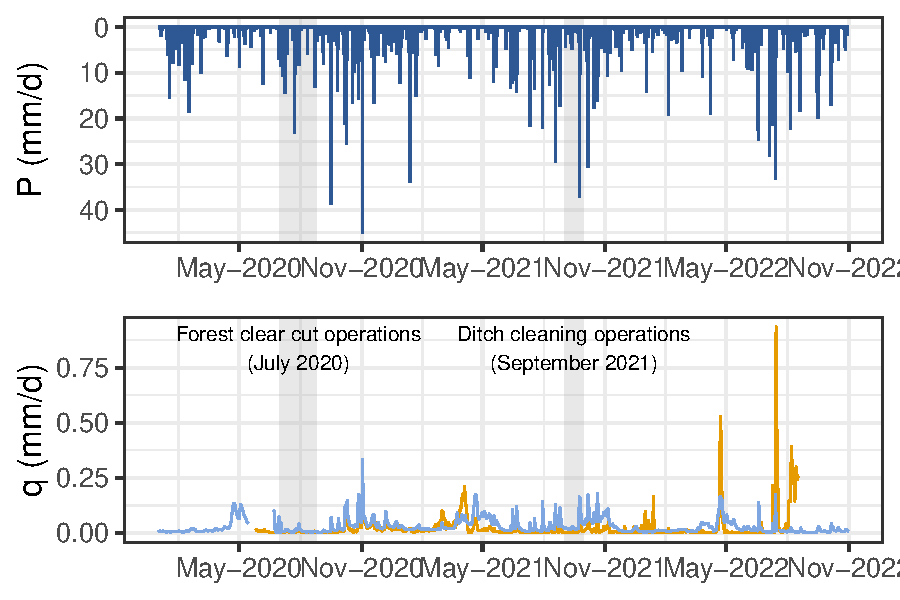
\includegraphics{index_files/figure-pdf/unnamed-chunk-2-1.pdf}

}

\caption{Precipitation and discharge timeseries}

\end{figure}%

\begin{figure}[H]

{\centering 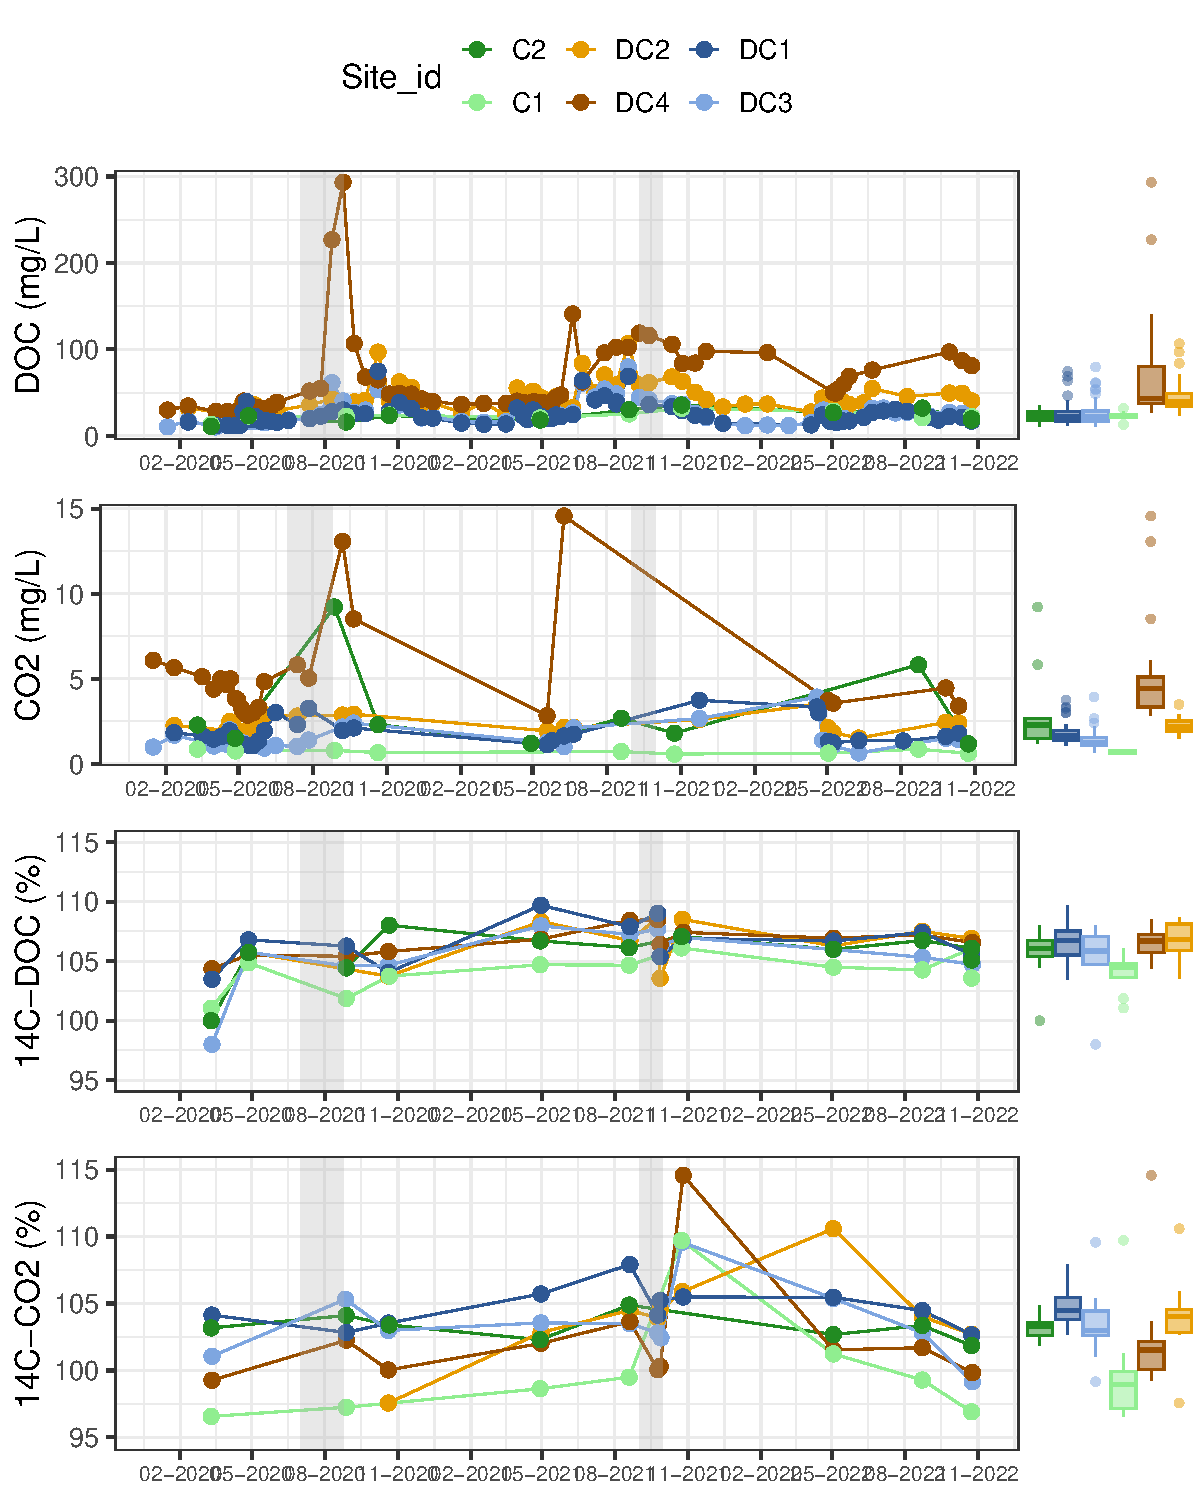
\includegraphics{index_files/figure-pdf/unnamed-chunk-3-1.pdf}

}

\caption{C concentration and radiocarbon content timeseries coloured by
sites}

\end{figure}%

\paragraph{Dunn's test \textbar{} ¹⁴C and {[}C{]} \textasciitilde{}
Site}\label{dunns-test-uxb9ux2074c-and-c-site}

\begin{verbatim}
# A tibble: 6 x 5
  Site  `[DOC]` `14C-DOC` `[CO2]` `14C-CO2`
  <fct>   <dbl>     <dbl>   <dbl>     <dbl>
1 C2       23.2      106.    2.29     103. 
2 C1       22.5      104.    0.73      99.0
3 DC2      39.1      107.    2.17     104. 
4 DC4      44.1      107.    4.43     102. 
5 DC1      21.4      107.    1.66     104. 
6 DC3      22.0      106.    1.26     103. 
\end{verbatim}

\begin{verbatim}
  Site [DOC] 14C-DOC [CO2] 14C-CO2
1   C2     a      ab   abc     abc
2   C1     a       a     d       a
3  DC2     b       b     a      bc
4  DC4     b       b     b      ab
5  DC1     a       b    ac       c
6  DC3     a      ab    cd     abc
\end{verbatim}

\begin{tcolorbox}[enhanced jigsaw, coltitle=black, opacitybacktitle=0.6, left=2mm, bottomtitle=1mm, colback=white, toprule=.15mm, arc=.35mm, toptitle=1mm, leftrule=.75mm, rightrule=.15mm, colbacktitle=quarto-callout-note-color!10!white, breakable, titlerule=0mm, bottomrule=.15mm, colframe=quarto-callout-note-color-frame, title=\textcolor{quarto-callout-note-color}{\faInfo}\hspace{0.5em}{Interpretation}, opacityback=0]

\textbf{Trend:}

\begin{itemize}
\item
  No obvious trends over time in C concentration or 14C content
\item
  There was a clear peak in DOC and CO2 concentration at DC4 during
  clearcut opperations.
\end{itemize}

\textbf{Differences between sites:}

\begin{itemize}
\item
  CO2 and DOC concentration at DC4 is consistently higher than the other
  sites, followed with DC2, and DC1 and DC3.
\item
  14C-DOC is not different across sites
\item
  14C-CO2 is significantly lower at DC4, followed with DC3 and DC2, DC1
  which is significantly higher
\end{itemize}

\end{tcolorbox}

\begin{tcolorbox}[enhanced jigsaw, coltitle=black, opacitybacktitle=0.6, left=2mm, bottomtitle=1mm, colback=white, toprule=.15mm, arc=.35mm, toptitle=1mm, leftrule=.75mm, rightrule=.15mm, colbacktitle=quarto-callout-warning-color!10!white, breakable, titlerule=0mm, bottomrule=.15mm, colframe=quarto-callout-warning-color-frame, title=\textcolor{quarto-callout-warning-color}{\faExclamationTriangle}\hspace{0.5em}{Q data}, opacityback=0]

The database contains DC3 and DC2 flow data, one ditch cleaned while the
other only clearcut. Other timeseries are incomplete.

\end{tcolorbox}

\subsection{Differences across
treatments}\label{differences-across-treatments}

Is there a significant change in the median \textsuperscript{14}C
content of CO\textsubscript{2} and DOC between sites or treatment, based
on their distribution ?

\begin{figure}[H]

{\centering 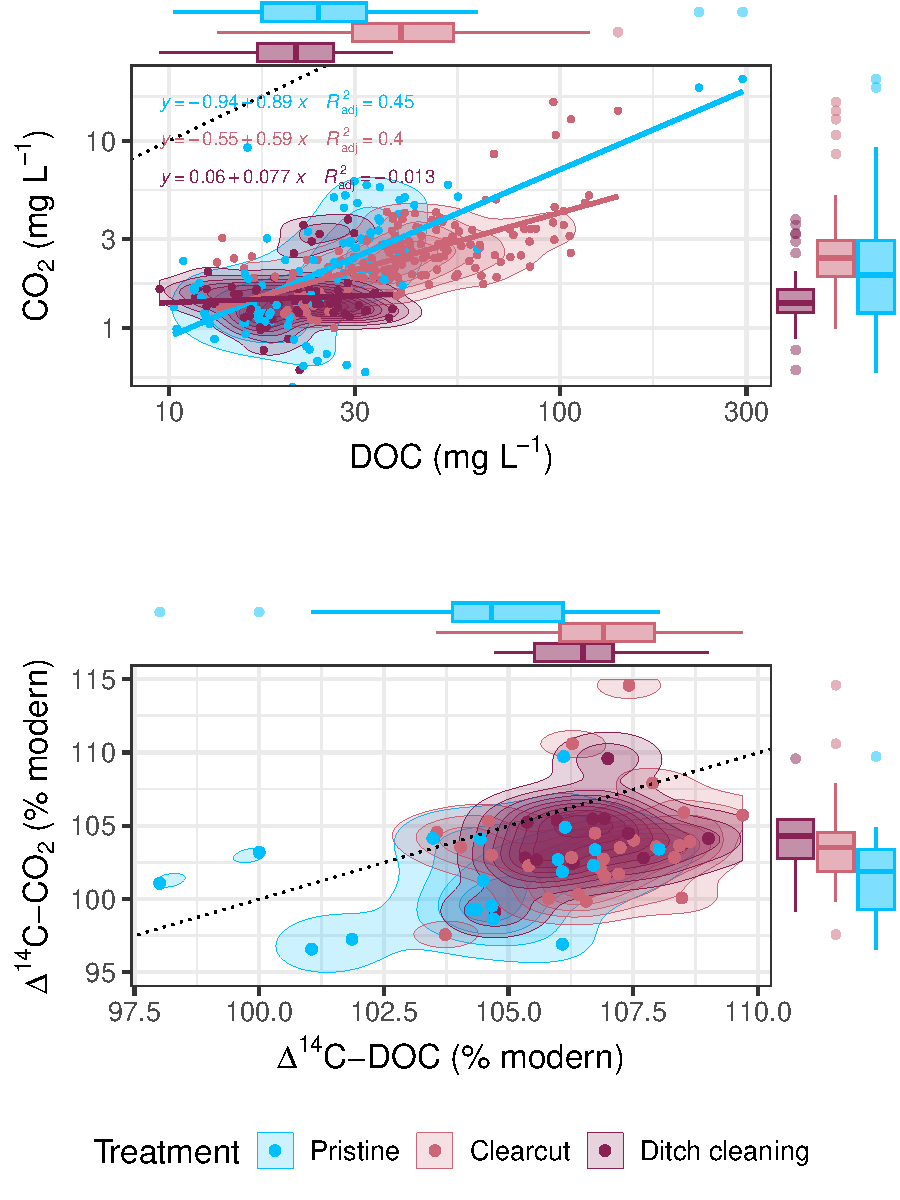
\includegraphics{index_files/figure-pdf/unnamed-chunk-6-1.pdf}

}

\caption{relationship between C concentration and radiocarbon content of
CO2 and DOC coloured by treatment}

\end{figure}%

ANOVA

\begin{verbatim}
ANOVA Table (type II tests)

                    Effect DFn DFd       F        p p<.05   ges
1           CO2_mgL_filled   1 317 459.060 1.36e-63     * 0.592
2                Treatment   2 317  29.092 2.51e-12     * 0.155
3 CO2_mgL_filled:Treatment   2 317   9.272 1.22e-04     * 0.055
\end{verbatim}

\paragraph{Dunn's test \textbar{} ¹⁴C et {[}C{]}\textasciitilde{}
Treatment}\label{dunns-test-uxb9ux2074c-et-c-treatment}

\begin{verbatim}
            Site 14C-DOC [DOC] 14C-CO2 [CO2]
1       Pristine       a     a       a     a
2       Clearcut       b     b      ab     a
3 Ditch cleaning       b     a       b     a
\end{verbatim}

\begin{tcolorbox}[enhanced jigsaw, coltitle=black, opacitybacktitle=0.6, left=2mm, bottomtitle=1mm, colback=white, toprule=.15mm, arc=.35mm, toptitle=1mm, leftrule=.75mm, rightrule=.15mm, colbacktitle=quarto-callout-note-color!10!white, breakable, titlerule=0mm, bottomrule=.15mm, colframe=quarto-callout-note-color-frame, title=\textcolor{quarto-callout-note-color}{\faInfo}\hspace{0.5em}{Interpretation}, opacityback=0]

\textbf{Treatment} \textbf{effect on C concentrations:}

\begin{itemize}
\item
  The DOC concentrations are significantly higher following clearcut
  treatment compared with ditchcleaned and pristine conditions (short
  term effect of ditch cleaning can compensate?)
\item
  The CO2 concentration do not differ significantly across treatment
\item
  The relationship between CO2 and DOC concentration is positive for
  pristine condition, but slope becomes less significant with clearcut
  and not significant (slope =0) with ditch cleaning. Hence the DOC
  concentration continues to vary across a wide range but the CO2
  becomes more stable.
\end{itemize}

\textbf{Treatment} \textbf{effect on 14 content}

\begin{itemize}
\item
  The \textsuperscript{14}C-DOC is significantly lower in the pristine
  (group a) compared with clearcut and ditch cleaning sites.
\item
  The \textsuperscript{14}C-CO\textsubscript{2} is doesn't differ
  significantly across treatments
\end{itemize}

\end{tcolorbox}

\subsection{Relationships - controls on C sources, age and
concentrations}\label{relationships---controls-on-c-sources-age-and-concentrations}

\subsubsection{Hydrological control over C
concentrations}\label{hydrological-control-over-c-concentrations}

Is the radiocarbon age or concentration of DOC and CO\textsubscript{2}
controled by runoff, and does this relationship changes after treatment?

\begin{figure}[H]

{\centering 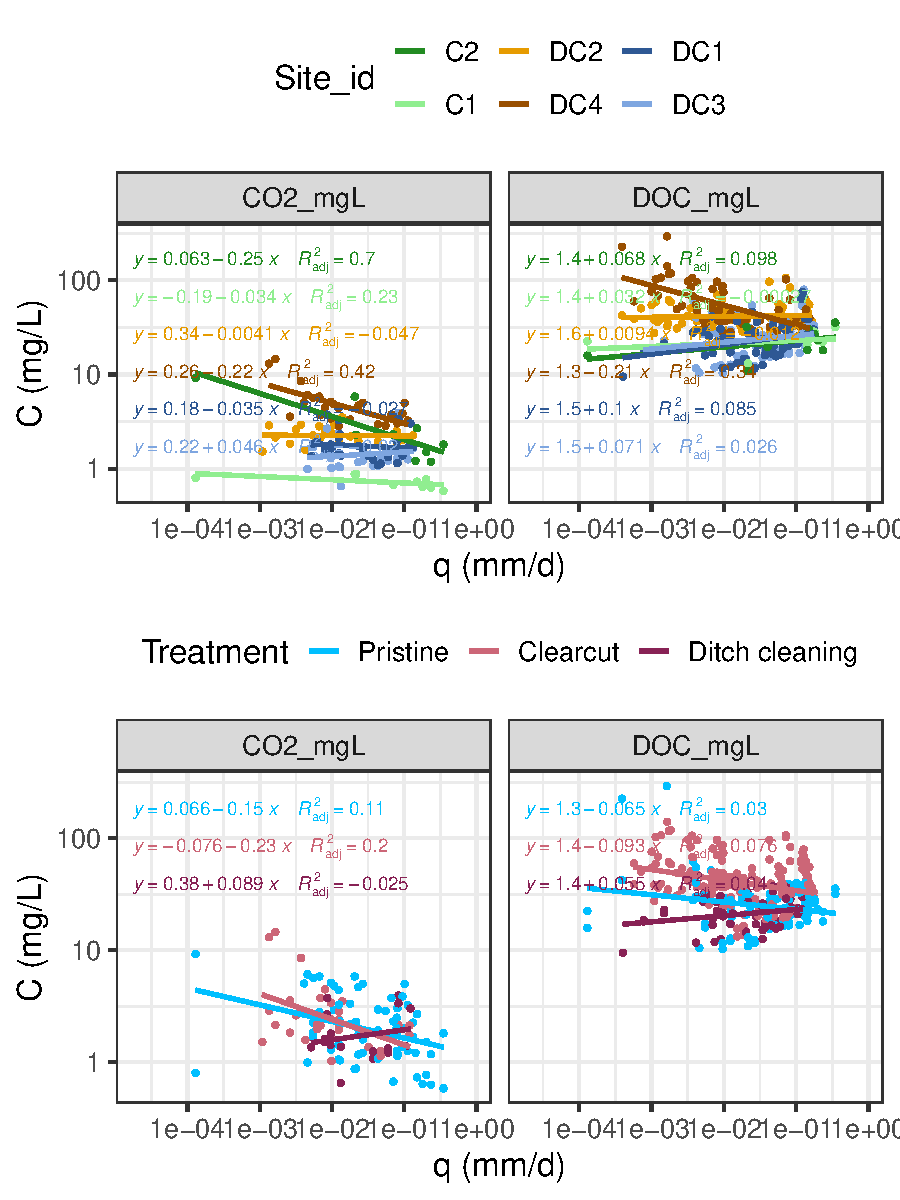
\includegraphics{index_files/figure-pdf/unnamed-chunk-9-1.pdf}

}

\caption{relationship between C concetration and discharge coloured by
site and treatment}

\end{figure}%

\paragraph{ANCOVA test}\label{ancova-test}

Is there a significant difference in the hydrological response of
\textbf{DOC} concentrations between \emph{Treatments or Sites}?

\begin{verbatim}
ANOVA Table (type II tests)

                 Effect DFn DFd      F        p p<.05   ges
1           q_md_filled   1 307  3.090 8.00e-02       0.010
2             Treatment   2 307 20.164 5.92e-09     * 0.116
3 q_md_filled:Treatment   2 307  0.389 6.78e-01       0.003
\end{verbatim}

\begin{verbatim}
ANOVA Table (type II tests)

               Effect DFn DFd      F        p p<.05      ges
1         q_md_filled   1 301  0.177 6.74e-01       0.000589
2             Site_id   5 301 26.589 3.00e-22     * 0.306000
3 q_md_filled:Site_id   5 301  5.631 5.58e-05     * 0.086000
\end{verbatim}

Is there a significant difference in the hydrological response of
\textbf{CO2} concentrations between \emph{Treatments or Sites}?

\begin{verbatim}
ANOVA Table (type II tests)

                 Effect DFn DFd     F     p p<.05   ges
1           q_md_filled   1 115 6.981 0.009     * 0.057
2             Treatment   2 115 1.602 0.206       0.027
3 q_md_filled:Treatment   2 115 1.804 0.169       0.030
\end{verbatim}

\begin{verbatim}
ANOVA Table (type II tests)

               Effect DFn DFd      F        p p<.05   ges
1         q_md_filled   1 109  7.711 6.00e-03     * 0.066
2             Site_id   5 109 20.742 1.64e-14     * 0.488
3 q_md_filled:Site_id   5 109  3.247 9.00e-03     * 0.130
\end{verbatim}

\begin{tcolorbox}[enhanced jigsaw, coltitle=black, opacitybacktitle=0.6, left=2mm, bottomtitle=1mm, colback=white, toprule=.15mm, arc=.35mm, toptitle=1mm, leftrule=.75mm, rightrule=.15mm, colbacktitle=quarto-callout-note-color!10!white, breakable, titlerule=0mm, bottomrule=.15mm, colframe=quarto-callout-note-color-frame, title=\textcolor{quarto-callout-note-color}{\faInfo}\hspace{0.5em}{Interpretation}, opacityback=0]

DOC and CO2 concentrations are not controled by Discharge

\begin{itemize}
\item
  Q \textbf{doesn't} have a significant effect on DOC concentration, but
  treatment and site do (intercept difference). Significant interaction
  between Q and Site (slope difference)
\item
  Q doesnt have a significant effect on CO2 concentration, nor does
  treatment. Site effect causes a signficant effect on intercept and
  slope (interaction)
\end{itemize}

\end{tcolorbox}

\subsubsection{\texorpdfstring{Hydrological controls over
\textsuperscript{14}C-content}{Hydrological controls over 14C-content}}\label{hydrological-controls-over-14c-content}

\begin{figure}[H]

{\centering 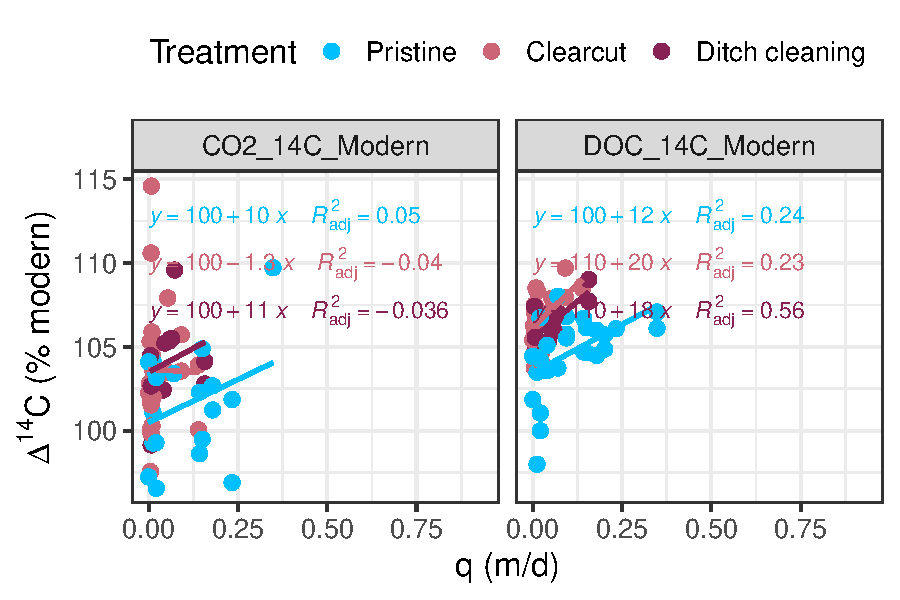
\includegraphics{index_files/figure-pdf/unnamed-chunk-12-1.pdf}

}

\caption{relationship between radiocarbon content of CO2 and DOC and
discharge, coloured by treatment}

\end{figure}%

\paragraph{ANCOVA test}\label{ancova-test-1}

Is there a significant difference in the hydrological response of
\textbf{14C-DOC} between \emph{Treatments}?

\begin{verbatim}
ANOVA Table (type II tests)

                 Effect DFn DFd      F        p p<.05   ges
1           q_md_filled   1  62 24.164 6.81e-06     * 0.280
2             Treatment   2  62 22.767 3.86e-08     * 0.423
3 q_md_filled:Treatment   2  62  0.684 5.08e-01       0.022
\end{verbatim}

Is there a significant difference in the hydrological response of
\textbf{14C-CO2} between \emph{Treatments}?

\begin{verbatim}
ANOVA Table (type II tests)

                 Effect DFn DFd     F     p p<.05   ges
1           q_md_filled   1  52 1.816 0.184       0.034
2             Treatment   2  52 4.062 0.023     * 0.135
3 q_md_filled:Treatment   2  52 0.237 0.790       0.009
\end{verbatim}

\paragraph{Linear mixed effect model}\label{linear-mixed-effect-model}

\begin{verbatim}

Call:
glm(formula = DOC_14C_Modern ~ q_md_filled * Treatment, data = DC_Q)

Coefficients:
                                     Estimate Std. Error t value Pr(>|t|)    
(Intercept)                         1.034e+02  4.459e-01 231.992  < 2e-16 ***
q_md_filled                         1.156e+04  3.017e+03   3.834 0.000298 ***
TreatmentClearcut                   2.739e+00  5.805e-01   4.718  1.4e-05 ***
TreatmentDitch cleaning             2.063e+00  8.153e-01   2.530 0.013958 *  
q_md_filled:TreatmentClearcut       8.617e+03  8.217e+03   1.049 0.298432    
q_md_filled:TreatmentDitch cleaning 6.027e+03  9.444e+03   0.638 0.525695    
---
Signif. codes:  0 '***' 0.001 '**' 0.01 '*' 0.05 '.' 0.1 ' ' 1

(Dispersion parameter for gaussian family taken to be 2.491009)

    Null deviance: 281.24  on 67  degrees of freedom
Residual deviance: 154.44  on 62  degrees of freedom
  (4341 observations deleted due to missingness)
AIC: 262.76

Number of Fisher Scoring iterations: 2
\end{verbatim}

\paragraph{ANCOVA test}\label{ancova-test-2}

Is there a significant difference in the hydrological response of
\textbf{14C-DOC} between \emph{Sites}?

\begin{verbatim}
ANOVA Table (type II tests)

               Effect DFn DFd      F        p p<.05   ges
1         q_md_filled   1  56 18.570 6.68e-05     * 0.249
2             Site_id   5  56  6.873 4.60e-05     * 0.380
3 q_md_filled:Site_id   5  56  1.194 3.24e-01       0.096
\end{verbatim}

\begin{tcolorbox}[enhanced jigsaw, coltitle=black, opacitybacktitle=0.6, left=2mm, bottomtitle=1mm, colback=white, toprule=.15mm, arc=.35mm, toptitle=1mm, leftrule=.75mm, rightrule=.15mm, colbacktitle=quarto-callout-note-color!10!white, breakable, titlerule=0mm, bottomrule=.15mm, colframe=quarto-callout-note-color-frame, title=\textcolor{quarto-callout-note-color}{\faInfo}\hspace{0.5em}{Interpretation}, opacityback=0]

\begin{itemize}
\item
  q has a significant effect on 14C-DOC, but not on 14C-CO2
\item
  (LME) there is a significant effect of both \textbf{Treatment}
  \textbf{14C-DOC} in the model (intercept differences), but no
  significant interaction (slope differences). No significant effect of
  Site\_id
\item
  The intercept shifts from 100\%modern in pristine sites, to
  110\%modern in clearcut+ditchcleaned sites.
\item
  Site\_id explains only 13\% of the variance (LME), not a significant
  predictor.
\end{itemize}

\end{tcolorbox}

\subsection{\texorpdfstring{Biological controls over
\textsuperscript{14}C-CO\textsubscript{2} - Keeling
plots}{Biological controls over 14C-CO2 - Keeling plots}}\label{biological-controls-over-14c-co2---keeling-plots}

\begin{figure}[H]

{\centering 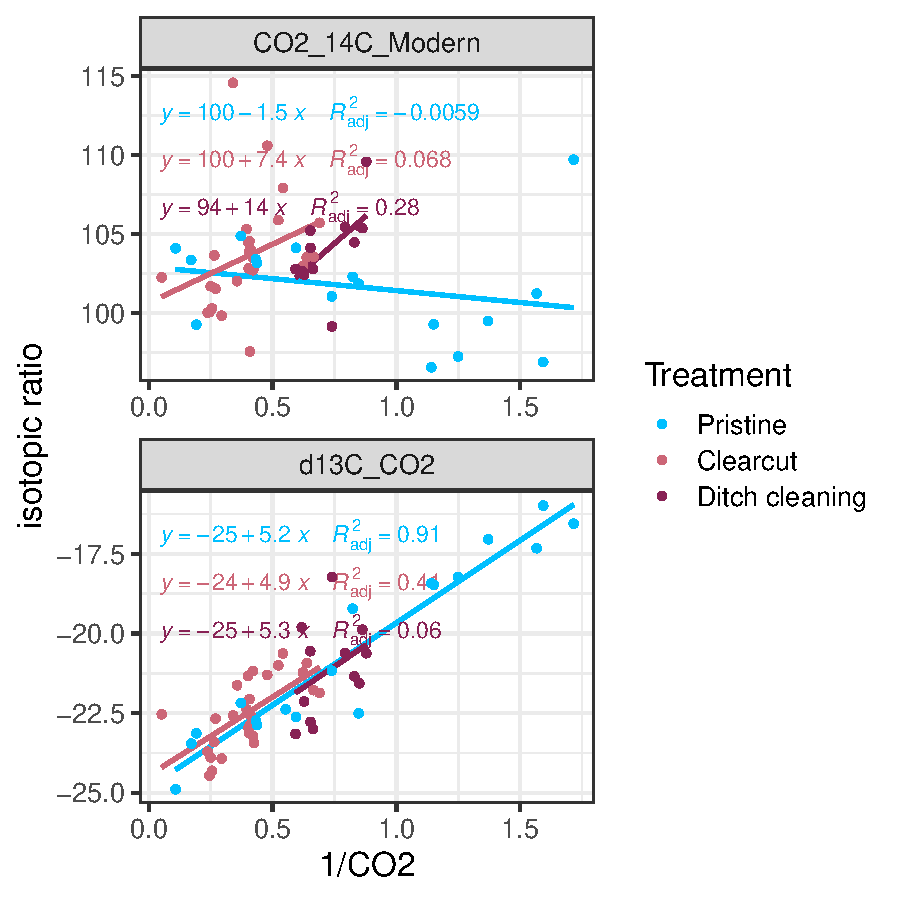
\includegraphics{index_files/figure-pdf/unnamed-chunk-17-1.pdf}

}

\caption{Keeling plot of CO2 isotope ratio, stable and radiogenic,
coloured by treatment}

\end{figure}%

\paragraph{ANCOVA test}\label{ancova-test-3}

Does the keeling relationship for \textbf{d13C-CO2} varies significantly
between treatment?

\begin{verbatim}
ANOVA Table (type II tests)

                            Effect DFn DFd       F        p p<.05      ges
1           CO2_mgL_filled_keeling   1  51 145.233 1.53e-16     * 0.740000
2                        Treatment   2  51   0.527 5.93e-01       0.020000
3 CO2_mgL_filled_keeling:Treatment   2  51   0.018 9.83e-01       0.000687
\end{verbatim}

Does the keeling relationship for \textbf{14C-CO2} varies significantly
between treatment?

\begin{verbatim}
ANOVA Table (type II tests)

                            Effect DFn DFd     F     p p<.05      ges
1           CO2_mgL_filled_keeling   1  50 0.014 0.907       0.000277
2                        Treatment   2  50 2.409 0.100       0.088000
3 CO2_mgL_filled_keeling:Treatment   2  50 3.347 0.043     * 0.118000
\end{verbatim}

\begin{tcolorbox}[enhanced jigsaw, coltitle=black, opacitybacktitle=0.6, left=2mm, bottomtitle=1mm, colback=white, toprule=.15mm, arc=.35mm, toptitle=1mm, leftrule=.75mm, rightrule=.15mm, colbacktitle=quarto-callout-note-color!10!white, breakable, titlerule=0mm, bottomrule=.15mm, colframe=quarto-callout-note-color-frame, title=\textcolor{quarto-callout-note-color}{\faInfo}\hspace{0.5em}{Interpretation}, opacityback=0]

\begin{itemize}
\item
  The keeling plot suggests that CO2 concentration has a significant
  effect on both d13C-value and 14C-concent, which supports the idea of
  a biological control.
\item
  But this relationship doesn't change signficantly with treatment.
  Perhaps the sample size is not enough to identify a meaningful effect
\item
  The d13C source of CO2 is (-25‰) (no signficant effect of slope or
  intercept across sites or treatment)
\item
  The 14C source of CO2 is between 99, 100m and 94. Which are large
  differences, but don't appear as significant effects in the model.
\end{itemize}

\end{tcolorbox}

\phantomsection\label{refs}
\begin{CSLReferences}{1}{0}
\bibitem[\citeproctext]{ref-campeau2019}
Campeau, A., K. Bishop, N. Amvrosiadi, M. F. Billett, M. H. Garnett, H.
Laudon, M. G. Öquist, and M. B. Wallin. 2019. {``Current Forest Carbon
Fixation Fuels Stream CO2 Emissions.''} \emph{Nature Communications} 10
(1). \url{https://doi.org/10.1038/s41467-019-09922-3}.

\bibitem[\citeproctext]{ref-campeau2017}
Campeau, Audrey, Kevin H. Bishop, Michael F. Billett, Mark H. Garnett,
Hjalmar Laudon, Jason A. Leach, Mats B. Nilsson, Mats G. Öquist, and
Marcus B. Wallin. 2017. {``Aquatic Export of Young Dissolved and Gaseous
Carbon from a Pristine Boreal Fen: Implications for Peat Carbon Stock
Stability.''} \emph{Global Change Biology} 23 (12): 5523--36.
\url{https://doi.org/10.1111/gcb.13815}.

\bibitem[\citeproctext]{ref-ledesma2013}
Ledesma, J. L. J., T. Grabs, M. N. Futter, K. H. Bishop, H. Laudon, and
S. J. Köhler. 2013. {``Riparian Zone Control on Base Cation
Concentration in Boreal Streams.''} \emph{Biogeosciences} 10 (6):
3849--68. \url{https://doi.org/10.5194/bg-10-3849-2013}.

\bibitem[\citeproctext]{ref-uxf6quist2014}
Öquist, M. G., K. Bishop, A. Grelle, L. Klemedtsson, S. J. Köhler, H.
Laudon, A. Lindroth, M. Ottosson Löfvenius, M. B. Wallin, and M. B.
Nilsson. 2014. {``The Full Annual Carbon Balance of Boreal Forests Is
Highly Sensitive to Precipitation.''} \emph{Environmental Science \&
Technology Letters} 1 (7): 315--19.
\url{https://doi.org/10.1021/ez500169j}.

\end{CSLReferences}




\end{document}
